%          be used with:
%          spconf.sty  - ICASSP/ICIP LaTeX style file, and
%          IEEEbib.bst - IEEE bibliography style file.
% --------------------------------------------------------------------------
\documentclass{article}
\usepackage{spconf,amsmath,epsfig}
\usepackage[english]{babel}

% Example definitions.
% --------------------
\def\x{{\mathbf x}}
\def\L{{\cal L}}

% Title.
% ------
\title{PEDESTRIAN DETECTION USING HAAR-LIKE FEATURES}
%
% Single address.
% ---------------
\name{Tim Besard, Ruben Schollaert, Dimitri Roose, Sebastiaan Labijn}
%\thanks{Thanks to University College Ghent for funding.}
\address{University College Ghent\\Applied Engineering\\Campus Schoonmeersen, Valentin Vaerwyckweg 1, 9000 Gent}
\begin{document}
%\ninept
%
\maketitle
%
\begin{abstract}
In this paper a solution for pedestrian detection is described using Haar-like features. It is being developed to be used in a tram collision avoidance project. 
\end{abstract}
%
\begin{keywords}
Pedestrian Detection, Haar-like Features, AdaBoost Classification
\end{keywords}
%
\section{Introduction}
\label{sec:intro}
Object detection is a very important element in computer vision areas. The goal is to find a predefined object in a set of images or video frames. This task can be fulfilled using template matching techniques extracting certain image features such as edges, color regions, textures and contours.
\par
Alas for complex objects such as pedestrians these features are hard to find due the great variety of instances of these pedestrians. This huge variety is caused by the following major problems~\cite{monteiro2006vision}:
\begin{itemize}
\item The size, color and style of pedestrian clothing are very diverse. Examples are shown in Figure~\ref{fig:people}.
\item Pedestrians are non-rigid bodies. Their shape and size differ greatly and therefore they are more complex then rigid objects.
\item Not only the pedestrians are part of the problem, but the background too. It can cause cluttering or can be mistaken for pedestrians due to its composition.
\item Illumination and weather conditions can lower the distinction between background and pedestrian.
\item Also the lack in motion due the slow speed of pedestrians hardens the possibility for them to be detected.
\end{itemize}
Instead of using the template matching approach, another possible method has been described by Viola and Jones~\cite{viola2001rapid} and extended by Lienhart and Maydt~\cite{lienhart2002extended}.
\section{How it works}
This approach uses statistical models, so called classifiers. These are created by extensive training using a pool of test images. These pools consists of positive and negative samples, respectively images that contain pedestrians and images that don't. 
From these sample images features will be extracted and the features which classify that pedestrians are selected. These are the so called Haar-like features. The general flow of this process is shown in Figure~\ref{fig:flowchart}.

\begin{figure}[h!]
	\centering
	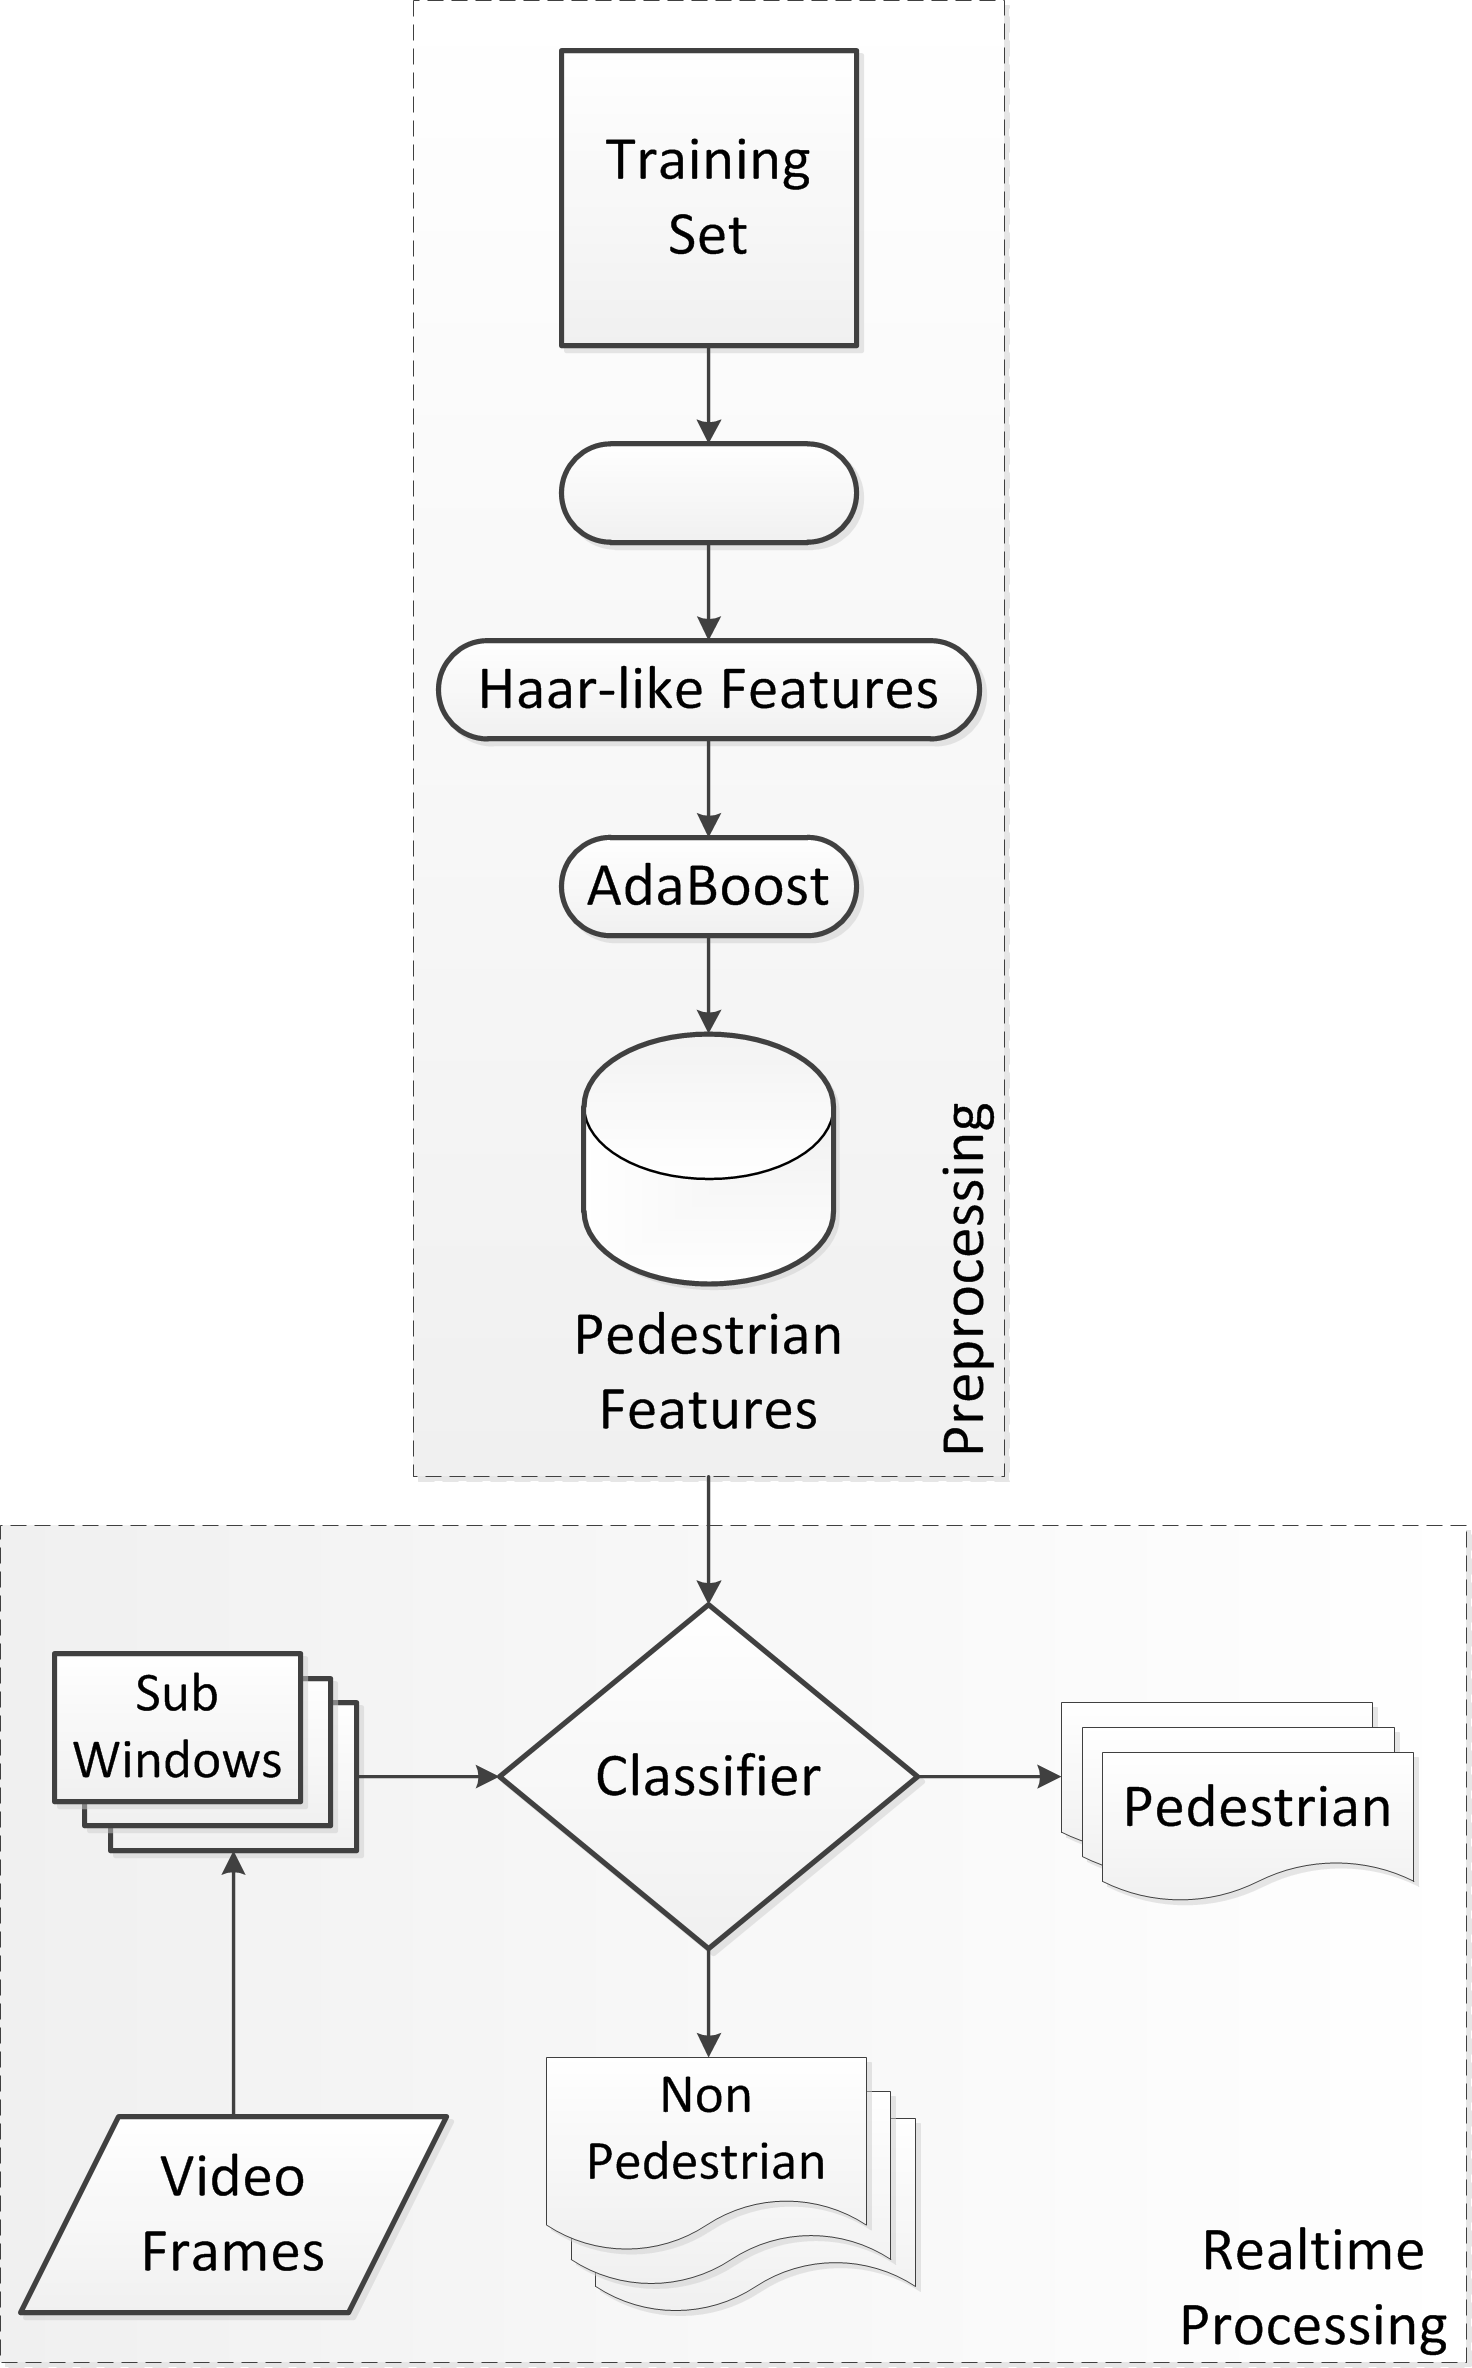
\includegraphics[scale=0.5]{HaarTrainingFlowChart.png}
	\caption{Flowchart for detecting pedestrians.}
	\label{fig:flowchart}
\end{figure}
\begin{figure}
	\centering
	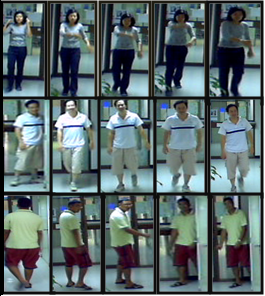
\includegraphics[scale=0.5]{People.png}
	\caption{Differences in size, color and clcothing of pedestrians.}
	\label{fig:people}
\end{figure}
\section{Haar-like features}
A Haar-like feature is represented by a template, its coordinate relative to the sub window and his size.
The template, a shape, is composed of two or three rectangles joined together. Each of these rectangles is colored black or white. Three of these Haar-like features are displayed in Figure~\ref{fig:features}. These rectangles can be turned horizontal, vertical or even  diagonal, an extension proposed in~\cite{lienhart2002extended}.

\begin{figure}[h!]
	\centering
	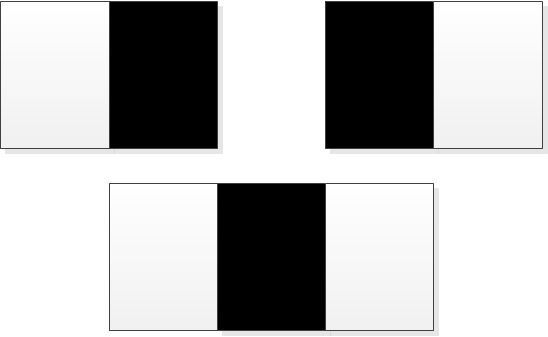
\includegraphics[scale=0.6]{Features.png}
	\caption{Prototypes of Haar-like features.}
	\label{fig:features}
\end{figure}

\par
For each feature a value is calculated for each position in the search sub window. These values sum up the pixel intensities in these regions and calculates the difference between them. This difference is then used to check whether the feature resembles with this position on the sub window.
\par
A sub window of an image contains a far larger amount of features than pixels. Therefore a mechanism is needed to select the most valuable ones.
\section{AdaBoost}
Once a machine learning system has a training set of positive and negative samples and a feature set, it can be invoked to fulfill the training of the classifier. Viola and Jones~\cite{viola2001rapid} used a variant of AdaBoost to both select a small set of features and to train the classifier. In its original form, the AdaBoost learning algorithm is used to boost the classification performance of a simple learning algorithm. AdaBoost is an algorithm which constructs a strong classifier as a combination of weak classifiers.
\par
Although each feature can be computed very efficiently, the computation of the complete feature set is unfeasible.
\par
Building the boosted classifiers takes the most time because it requires a lot of training data and iterations in the AdaBoost algorithm. Once these classifiers are built, the detection is capable of processing images extremely rapidly and achieving high detection rates~\cite{viola2001rapid}.
\section{Training a cascade of classifiers}
Each stage of the cascade of classifiers consists of a classifier which has been trained by the above AdaBoost algorithm. The general structure of a cascade is shown in Figure~\ref{fig:cascade}. It can be seen as a degenerated decision tree where at  each stage a classifier is trained to detect almost all objects of interest while rejecting fractions of non-object patterns.~\cite{viola2001rapid}~\cite{viola2005detecting}
\begin{figure}[h!]
	\centering
	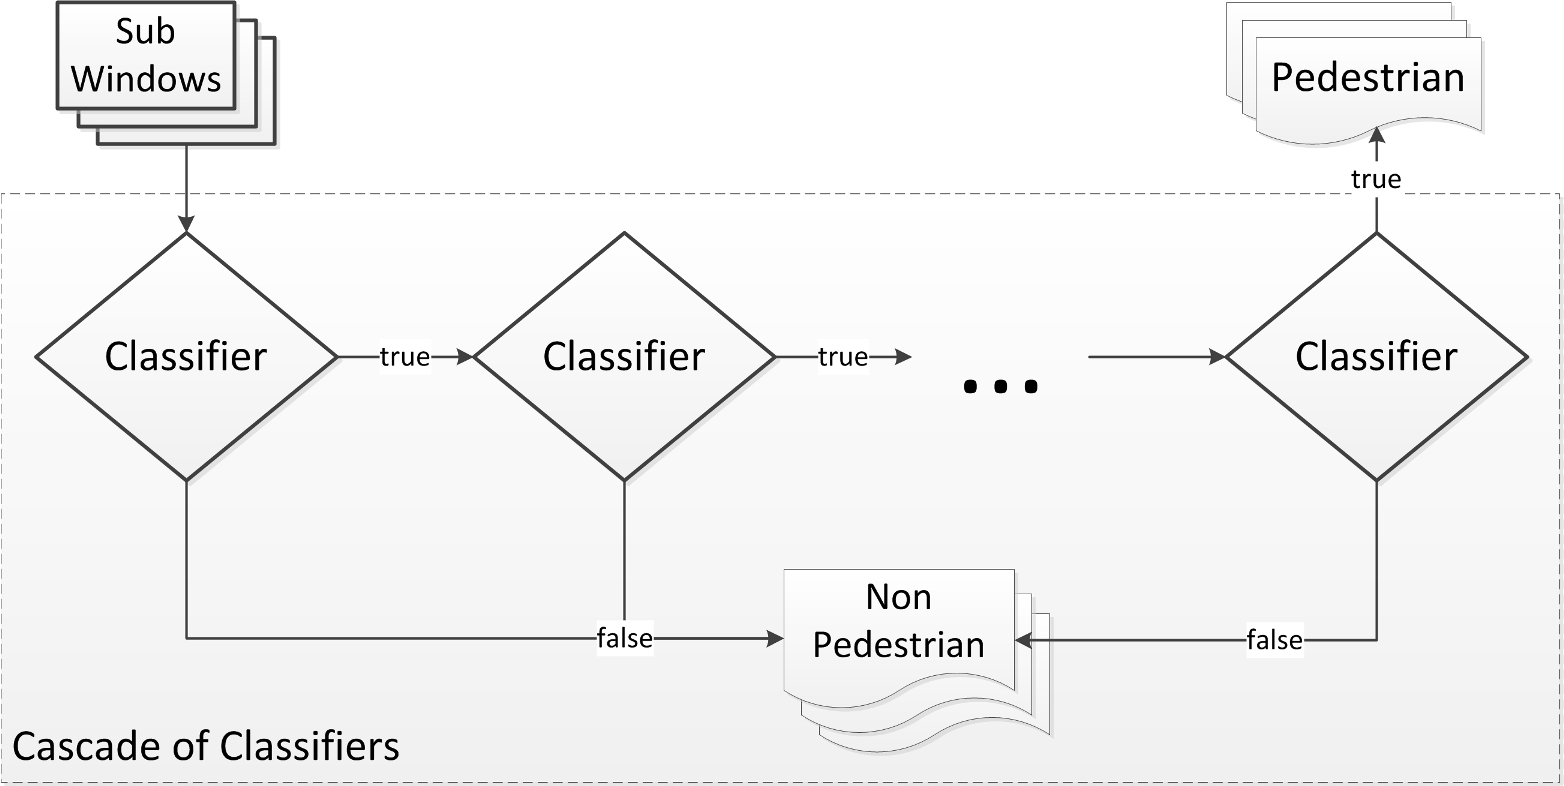
\includegraphics[scale=0.6]{Cascade.png}
	\caption{A cascade of classifiers.}
	\label{fig:cascade}
\end{figure}
\par
In practice a very simple framework is used to produce an effective classifier which is highly efficient. Each stage in the cascade reduces the false positive rate as well as the detection rate. A target is selected for the minimum reduction in false positives and the maximum decrease in detection. Each stage is trained by adding features until the target detection and false positives rates are met. Stages are added until the overall target for false positive and detection rate is met. 
\par
To have a highly efficient outcome a goal is set at the beginning, this goal contains the number of false positives and the detection rate. After this goal is set, a new stage with new weak classifiers is added to the cascade. After every stage the new cascade of classifiers is tested on a validation set. If the goal is not yet reached, new stages are added over and over again.~\cite{monteiro2006vision}
\par
Using this framework the simpler classifiers go first. They will then reject the majority of the negative matches. When a window passes these simpler classifiers, more complex ones are used. This causes a lower false positive rate. The key is to decrease the false positive rate more rapidly than the detection rate.
\par
To create a successful cascade of classifiers a lot of samples are required. These samples contain images from pedestrians in all possible poses, sizes and with different clothing. A large number of samples are required for a good detection rate.
\par
A pedestrian detection cascade file, as delivered with OpenCV, contains 30 stages. Each stage contains 40 features. 
\section{OpenCV Haartraining}
To create and test the cascade of boosted classifiers based on Haar-like features we are using OpenCV \cite{opencv_library}. OpenCV provides us programs that we can use to create our own classifiers.
\subsection{Create samples}
Before we can start creating samples we need positive images, these are images which contain pedestrians without much variations in the illumination, if there are too many variations the resulting detector will not work well. Besides the positive images we also need negative images and testing images. The testing images are images combined with the location of the pedestrians. We used the CBCL PEDESTRIAN DATABASE \#1 from MIT which contains 924 images.~\cite{pedestrianset}
From one image we can create several samples by using distortion, we can use the \texttt{createsamples} program delivered by OpenCV for this. For example:
\texttt{\begin{tabbing}
createsamples \= -img image.png \\
\> -num 10 -bg negatives.dat \\
\> -vec samples.vec \\
\> -w 64 -h 128
\end{tabbing}}
This will generate ten samples out of one image. The file \texttt{negatives.dat} is a file containing a list of the negative images used.
For the test images we need to create a file which includes the location of the pedestrian in each image. This file will just hold the x and y coordinates in combination with the height and width of the pedestrian.
After these steps we can start creating the testing samples, these are created as follows:
\texttt{\begin{tabbing}
createsamples \= -img image.png \\
\> -num 10 -bg negatives.dat \\
\> -info test.dat \\
\> -maxxangle 0.6 -maxyangle 0 \\
\> -maxzangle 0.3 -maxidev 100 \\
\> -bgcolor 0 -bgthresh 0
\end{tabbing}}
This will generate cropped pedestrians placed on top of negative samples as output. A description file with the coordinates of the cropped pedestrian in the new image will also be available.
\subsection{Train}
To train our classifier we can use the \texttt{haartraining} utility. The following training takes about four days:
\texttt{\begin{tabbing}
haartraining \= -data haarcascade \\
\> -vec samples.vec \\
\> -bg negatives.dat \\
\> -nstages 20 -nsplits 2 \\
\> -npos 5000 -nneg 2500 \\
\> -w 20 -h 80 -nonsym \\
\> -mem 512 -mode ALL
\end{tabbing}}
We use the \texttt{-nonsym} parameter because people don't have a symmetric body structure in all poses. If we would be making classifiers for a symmetric object we would use the default, so only half of the image will be processed  thus speeding up the training. We also specified the \texttt{-mode ALL}, this means the Haar-training will look for all Haar-like features, default will only look for upright features.
Increasing the number of stages (\texttt{-nstages 20}) will not necessarily produce a better result. If the default threshold of minimum 99.5\% hit rate or the maximum false alarm of 50\% is reached, the training will stop.
When the training is finished, OpenCV will generate an XML output file.
\subsection{Test}
OpenCV also has a program to test the performance of the generated classifiers. This program is called \texttt{performance}. Testing the XML can be done like this:
\texttt{\begin{tabbing}
performance \= -data haar-cascade.xml \\
\> -info tests.dat \\
\> -ni
\end{tabbing}}
The \texttt{tests.dat} file contains a list of testing images and the \texttt{ni} parameter is used so the performance-utility will not output any detection images. The performance-utility will then output the number of correct detections, the number of missed or false negatives and the number of false positives.
\section{Experimental results}

\begin{figure}[h!]
	\centering
	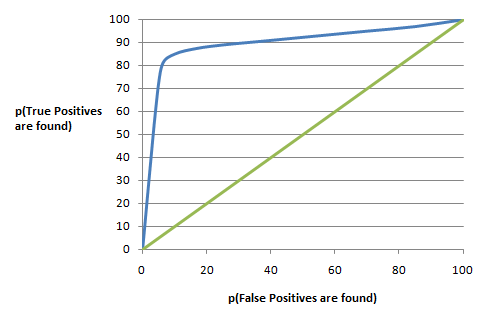
\includegraphics[scale=0.68]{roc.png}
	\caption{ROC of the test results}
	\label{fig:roc}
\end{figure}

To test the detector created by OpenCV we used a set of 40 positive images and 60 negative images. A Receiver Operating Characteristic curve showing the performance of our detector on this test set is shown in Figure \ref{fig:roc}. We can hereby conclude that a small increase in false positives detected will result in a very steep increase in number of true positives found at start. But any increase past the 20\% false postives mark will result a smaller amount of increased true positive cases then number of extra false positives.

We also tested the speed and number of positive and negative detections when reducing the orignal size (1280x720px) of the images to 80\%, 60\% and 40\%. The results of this test can be found in Table \ref{table:test}. As you can see from these results the bigger the size of the image is the more people are detected but also the detection time increases. Going from 40\% to 100\% image size gives us a gain of 25\% more people detected. It does increase multiply the detection time by 800\% from 100ms to 900ms. The number of false detections is multiplied by 5 for that matter.

\begin{table}[h!]
\centering
\scalebox{0.9}{%
    \begin{tabular}{ | c | c | c | c |}
    \hline
    Image size & Detection time & People detected & False detections \\ \hline
    100\%  & 900ms & 85\% & 10\% \\  \hline
    80\%   & 600ms & 85\% & 5\% \\  \hline
    60\%   & 280ms & 80\% & 3\% \\  \hline
    40\%   & 100ms & 60\% & 2\% \\ \hline
    \end{tabular}}
\caption{Test results when resizing the image}
\label{table:test}
\end{table}

Figure \ref{fig:pdetection1} and \ref{fig:pdetection2} show the output of our detector on some of the test images.
\begin{figure}[h!]
	\centering
	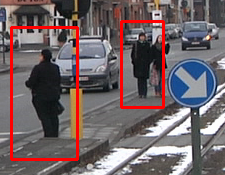
\includegraphics[scale=0.60]{peopledetection1.png}
	\caption{People detection: two people as a group}
	\label{fig:pdetection1}
\end{figure}
\begin{figure}[h!]
	\centering
	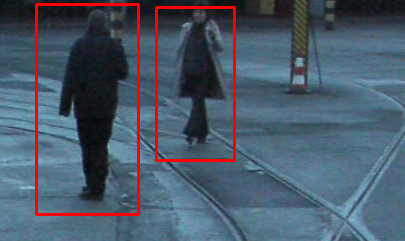
\includegraphics[scale=0.4]{peopledetection2.png}
	\caption{People detection: two seperate}
	\label{fig:pdetection2}
\end{figure}
\section{Conclusion}
In this paper we discussed a method for pedestrian detection to be used in a tram collision avoidance project. By using a boosted cascade of Haar-like features this is made possible. After preprocessing the cascade of classifiers the detection is able to be used in real time.
\bibliographystyle{IEEEbib}
\bibliography{bibliografie}
\end{document}
